%%%%%%%%%%%%%%%%%%%%%%%%%%%%%%%%%%%%%%%%%%%%%%%%%%%%%%%%%%%%%%%%%
\chapter{MINIATURE RF ION THRUSTER DESIGN}\label{ch:Ch3}
%%%%%%%%%%%%%%%%%%%%%%%%%%%%%%%%%%%%%%%%%%%%%%%%%%%%%%%%%%%%%%%%%
% \vspace*{-12pt} % If no text above section, use this vspacing to lift the whole part to the proper starting point - SBÖ
% % \section{Design Parameters}
Thruster is designed to be mainly operated by using Argon propellant. Design of the thruster includes discharge chamber, ion extraction grids, RF coil and other support elements such as rods and screws. Most dominant factor in thruster design is limitations imposed by the cubesat standarts. Entire thruster must be smaller than 10 centimeters in diameter in order to fit longitudinally into a cubesat but also must be large enough to ease manufacturing of sensitive thruster elements such as ion extraction grids and discharge chamber. Design of the thruster is made using CATIA V5. For RF system analysis ANSYS HFSS was used.
% In this chapter performed sizing studies and subsequent thruster design will be explanined.

\section{Sizing}
Thruster is designed to fit into a 3U sized (approximately 30cm x 10cm x 10cm) cubesat. Chassis and dimensions of such cubesat is shown in figure \ref{fig:3Udims}.

\begin{figure}[ht]
    \centering
    \includegraphics[scale=0.5]{fig/3Udims.png}
    \caption{3U cubesat structure with dimensions}
    \label{fig:3Udims}
\end{figure}

Based on dimensions shown in figure \ref{fig:3Udims} thruster diameter has to be smaller than 98.4 millimeters in diameter. There have been RF ion thrusters designed for cubesat applications in the past that had diameters smaller than 10 cm. BUSEK company have developed a RF ion thruster named BIT-3 which is shown in figure \ref{fig:BIT3}. This thruster has a 3cm grid from which it gets its name. BIT-3 is slated to be launched into Lunar orbit aboard a 6U sized cubesat named LunarCube in near future. 

\begin{figure}[ht]
    \centering
    \includegraphics[scale=.8]{fig/BIT3.png}
    \caption[BIT-3 next to US 1\$ coin]{BIT-3 next to US 1\$ coin\cite{tsay2015lunarcube}}
    \label{fig:BIT3}
\end{figure}

BUSEK has also developed a smaller thruster called BIT-1 shown in figure \ref{fig:BIT1}. This thruster is designed to support Laser Interferometer Space Antenna(LISA) mission set to launch in 2037. Primary purpose of BIT-1 is to provide precise attitude control\cite{tsay2012micro}. 

\begin{figure}[ht]
    \centering
    \includegraphics{fig/BIT1.png}
    \caption[BIT-1 next to US 1\$ coin]{BIT-1 next to US 1\$ coin\cite{tsay2012micro}}
    \label{fig:BIT1}
\end{figure}

Based on BUSEK's work and size of cubesat structure, sizing limitations for thruster are set to be between 10 millimeters to 98.4 millimeters. Considering the mechanical manufacturing convenience it was decided that overall thruster diameter shall be 94 millimeters. All subsystems of thruster have been designed accordingly. 
% RIT series developed by Giessen University and BIT series developed by BUSEK company can be shown as examples. 

\section{Plasma Generation System}
Plasma generation system consists of an RF coil to broadcast the signal and a discharge chamber to contain plasma as mentioned earlier in chapter \ref{ch:2_background}. 
\subsection{Discharge Chamber}
Material for discharge chamber is chosen as glass due to its ease of handling and accesibility. It was designed to consist wide and thin sections. Thin section will act as a channel through which the propellant will be fed into the wide section. Plasma will be created and sustained within the wide section. Approximate dimensions of discharge chamber is listed in table \ref{table:DC_params}. CAD and manufactured model of discharge chamber can be seen in figures \ref{fig:DC_cad} and \ref{fig:DC_real}. Approximations are the result of the relatively high manufacturing tolerances of glass production. 

\begin{table}[ht]
    \centering
    \begin{tabular}{||c|c||}
        \hline
        \textbf{Parameter} & \textbf{Approximate Value(mm)} \\
        \hline
        Total Length & 122 \\
        \hline
        Thin Section Lenght & 65 \\
        \hline
        Thin Section Outer Diameter & 6.35 \\
        \hline
        Wide Section Lenght & 57 \\
        \hline
        Wide Section Outher Diameter & 40 \\
        \hline
        Overall Thickness & 2 \\
        \hline
    \end{tabular}
    \caption{Parameters of Discharge Chamber}
    \label{table:DC_params}
\end{table}
 
\begin{figure}[ht]
    \centering
    \includegraphics[scale=.45]{fig/DC_CAD.jpg}
    \caption{CAD of discharge chamber}
    \label{fig:DC_cad}
\end{figure}

\begin{figure}[ht]
    \centering
    \includegraphics[scale=.35]{fig/DC_real.jpeg}
    \caption{Real model of discharge chamber}
    \label{fig:DC_real}
\end{figure}

\newpage
\subsection{RF Coil}
Due to skin depth effect RF signal is carried close to conductive material surface. Material selection for RF coil is made as copper. At 13.56MHz skin depth of copper is calculated to be 17.7$\mu$m\cite{bowick2011rf}. This fact allows the use of a tube instead of a solid transmission line. Using a tube is beneficial since it saves from material and it can be easily shaped into a coil. Parameters regarding the coil is given in table \ref{table:RFcoil_params}. CAD and real models of coil can be seen in figures \ref{fig:coil_CAD} and \ref{fig:coil_real}.
\newpage
\begin{table}[ht]
    \centering
    \begin{tabular}{||c|c||}
        \hline
        \textbf{Parameter} & \textbf{Value} \\
        \hline
        Inner Diameter & 4.7 mm\\
        \hline
        Outer Diameter & 2 mm \\
        \hline
        Overall length & 78.2 mm \\
         \hline
        Number of Turns & 5 \\
        \hline
    \end{tabular}
    \caption{Parameters of RF Coil}
    \label{table:RFcoil_params}
\end{table}

\begin{figure}[ht]
    \centering
    \includegraphics[scale=0.35]{fig/coil_CAD.png}
    \caption{CAD of RF coil}
    \label{fig:coil_CAD}
\end{figure}

\begin{figure}[ht]
    \centering
    \includegraphics[scale=0.35]{fig/realcoil.jpeg}
    \caption{RF coil}
    \label{fig:coil_real}
\end{figure}

\subsubsection{Coil Impedance}

Impedance is defined as the resistance of a conductor to the alternating current flowing through the said conductor. It is defined as the cumulative   effect of theresistance and reactance values of the circuit and similar to the resistance it is defined in ohm ($\Omega$) SI units. It is dependent on operating frequency.

Impedance value of the RF coil is important. A mismatch between the impedance values of the source and load, in this case RF coil, greatly hampers signal transmission. Details regarding the impedance mismatch and matching networks is provided in chapter \ref{ch:Ch4_mn}.\\

Impedance value measurements of the RF coil is performed via Siglent SVA 1032X Signal \& Vector Network Analyzer (VNA). Measurements can be displayed on the Smith chart. Smith chart is a circular shaped tool that is divided into inductive and capacitive regions shown in figure \ref{fig:smith_ex}. The impedence value measurements are inscripted onto the chart based on its imaginary (reactance) and real (resistance) values. Based on the reading an electrical circuit can be easily designed to bring the impedance value reading to the center of the Smith chart thus match the signal. 

\begin{figure}
    \centering
    \includegraphics{fig/smithchart_ex.png}
    \caption{Smith chart with descriptions}
    \label{fig:smith_ex}
\end{figure}
\newpage
RF coil is connected to the vector network analyzer's trace generation port via a split RF cable as shown in figure \ref{fig:antenna_meas}.

\begin{figure}[ht]
    \centering
    \includegraphics[scale=0.3,angle=90]{fig/antenna_meas.jpeg}
    \caption{Antenna connection to VNA}
    \label{fig:antenna_meas}
\end{figure}

Impedance value is measured at 13.56MHz. Result is shown in figure \ref{fig:smithchart_meas}

\begin{figure}[ht]
    \centering
    \includegraphics[scale=0.75]{fig/smithchart_meas.png}
    \caption{Impedance measurement of the RF coil}
    \label{fig:smithchart_meas}
\end{figure}
 
As can be seen from figure \ref{fig:smithchart_meas} impedance value for RF coil is far from ideal and an antenna tuner is needed.

\newpage
\section{Ion Extraction System} 
A pair of grids made out of stainless steel is designed and manufactured to act as the ion extraction system. In order to achieve optimum perveance, distance between grids and aperture diameters of screen and accel grids have to be determined. Literature survey on previous missions that include RF ion thrusters has been conducted to serve as a basis for grid distancing and aperture sizing. Results are provided in graph form in figure \ref{fig:farnellgrids}. 

\begin{figure}[ht]
    \centering
\includegraphics{fig/farnellgrids.png}
\caption[Geometrical parameters of RF ion grids in various missions]{Geometrical parameters of RF ion grids in various missions\cite{farnell2007performance}}
\label{fig:farnellgrids}
\end{figure}

Additionally grid parameters of BURFIT-80 have been taken into account since the thruster is proven to perform nominally. Based on these informations thicknesses of both grids have been determined to be 0.5 millimeters. Aperture diameteres of screen and accel grids are set to be 2.2 millimeters and 1.2 millimeters respectively. Distance between grids is set to be 1 millimeters.
\newpage
Laser cutting have been used to manufacture the grids. Four sets of pairs with different aperture numbers and different types of steel have been designed. For each grid an ear-like protrusion have been added to ease accesibility for electrical connections. Parameters, CAD and real model of first set of pairs is shown in table \ref{table:params_firstset}, figures \ref{fig:cad_firstset} and \ref{fig:real_firstset} respectively.

\begin{table}[ht]
    \centering
    \begin{tabular}{||c|c|c||}
        \hline
        \textbf{Parameter} & \textbf{Screen Grid} & \textbf{Accel. Grid} \\
        \hline
        Material & Steel SS304 & Steel SS304 \\
        \hline
        Outer diameter & 32 mm & 32 mm \\
        \hline
        Number of apertures & 91 & 91 \\
        \hline
        Aperture diameter & 2.2 mm & 1.2 mm \\
        \hline
        Thickness & 0.5 & 0.5 \\
        \hline
        Center-to-center distance between apertures & 3.2 mm & 3.2 mm \\
        \hline      
    \end{tabular}
\caption{Parameters of first set of grids}
\label{table:params_firstset}
\end{table}

\begin{figure}[ht]
    \centering
    \includegraphics[scale=.3]{fig/screen_6_cad.png}
    \includegraphics[scale=.3]{fig/accel_6_cad.png}
    \caption{CAD of screen(\textit{left)} and accel(\textit{right}) grids belonging to first set}
    \label{fig:cad_firstset}
\end{figure}

\begin{figure}[ht]
    \centering
    \includegraphics[scale=.08]{fig/screen_6_real.jpg}
    \includegraphics[scale=.08]{fig/accel_6_real.jpg}
    \caption{Real model of screen(\textit{left)} and accel(\textit{right}) grids belonging to first set}
    \label{fig:real_firstset}
\end{figure}

\newpage

Second set of grids with decreased number of apertures have been designed in order to ease manufacturing process and possibly reduce imperfections caused by production. Parameters, CAD and real model of first set of pairs is shown in table \ref{table:params_firstset}, figures \ref{fig:cad_firstset} and \ref{fig:real_firstset} respectively.

\begin{table}[ht]
    \centering
    \begin{tabular}{||c|c|c||}
        \hline
        \textbf{Parameter} & \textbf{Screen Grid} & \textbf{Accel. Grid} \\
        \hline
        Material & Steel SS304 & Steel SS304 \\
        \hline
        Outer diameter & 32 mm & 32 mm \\
        \hline
        Number of apertures & 61 & 61 \\
        \hline
        Aperture diameter & 2.2 mm & 1.2 mm \\
        \hline
        Thickness & 0.5 & 0.5 \\
        \hline
        Center-to-center distance between apertures & 4.2 mm & 4.2 mm \\
        \hline      
    \end{tabular}
\caption{Parameters of second set of grids}
\label{table:params_secondset}
\end{table}

\begin{figure}[ht]
    \centering
    \includegraphics[scale=.25]{fig/screen_5_cad.png}
    \includegraphics[scale=.25]{fig/accel_5_cad.png}
    \caption{CAD of screen(\textit{left)} and accel(\textit{right}) grids belonging to second set}
    \label{fig:cad_secondset}
\end{figure}

\begin{figure}[ht]
    \centering
    \includegraphics[scale=.35]{fig/screen_5_real.jpeg}
    \includegraphics[scale=.37]{fig/accel_5_real.jpeg}
    \caption{Real model of screen(\textit{left)} and accel(\textit{right}) grids belonging to second set}
    \label{fig:real_secondset}
\end{figure}

After the manufacture of first two sets imperfections, burrs and scorch marks have been observed around the apertures of the grids which are shown in figures \ref{fig:imperfect1} and \ref{fig:imperfect2}. 

\begin{figure}[ht]
    \centering
    \includegraphics[scale=0.25]{fig/imperfect2.jpeg}
    \caption{Imperfections on grids}
    \label{fig:imperfect1}
\end{figure}

\begin{figure}[ht]
    \centering
    \includegraphics[scale=0.25]{fig/imperfect1.jpeg}
    \caption{Close-up on imperfections on grids}
    \label{fig:imperfect2}
\end{figure}
\newpage
These imperfections are the result of usage of oxygen in the laser cutting process. Imperfections increase the risk of arc forming between grids when high voltage is introduced. In order to get rid of such impurities two additional sets, third and fourth, have been manufactured using a more durable kind of steel, SS316, and nitrogen instead of oxygen during laser cutting.  Apart from the differences in manufacturing process, parameters of third and fourth sets are identical to first and seconds sets respectively.

\begin{figure}[ht]
    \centering
    \includegraphics[scale=0.25]{fig/imperfect3.jpeg}
    \caption{Close-up on grids manufactured by nitrogen laser cutting}
    \label{fig:imperfect3}
\end{figure}

Result of nitrogen laser cutting is shown in figure \ref{fig:imperfect3} which shows a clear improvement regarding imperfections. Summary of designed grid parameters is provided in table \ref{table:gridparamsum}

\begin{table}[ht]
    \centering
    \begin{tabular}{||p{2cm}|p{2.2cm}|p{2.2cm}|p{2.5cm}|p{2.5cm}|p{2.7cm}||}
        \hline
        \textbf{Grid Set} & \textbf{Material} & \textbf{Number of Apertures} & \textbf{Screen Grid Aperture Dia.} & \textbf{Accel Grid Aperture Dia.} & \textbf{Distance Between Grids} \\
        \hline
        First Set & SS304 Steel & 91 & 2.2 mm & 1.2 mm & 1 mm \\
        \hline
        Second Set & SS304 Steel & 61 & 2.2 mm & 1.2 mm & 1 mm \\
        \hline
        Third Set & SS316 Steel & 91 & 2.2 mm & 1.2 mm & 1 mm \\
\hline
Fourth Set & SS316 Steel & 61 & 2.2 mm & 1.2 mm & 1 mm\\
\hline
    \end{tabular}
    \caption{Grid design parameters summary}
    \label{table:gridparamsum}
\end{table}
% \section{Support Structure}

\section{Thruster Assembly}
Grids, discharge chamber and RF coil are assembled together as shown in figures \ref{fig:thrusterassmgencad} and \ref{fig:thrusterassmgenreal}.

\begin{figure}[ht]
    \centering
    \includegraphics[scale=0.35]{fig/assm/assm_general.png}
    \caption{CAD of thruster assembly}
    \label{fig:thrusterassmgencad}
\end{figure}


\newpage

Exploded view of thruster design and explanation for each element is shown in figure \ref{fig:thrusterassmexp}. 

\begin{figure}[ht]
    \centering
    \includegraphics[width=\linewidth]{fig/assm/assm_exploded_ps.png}
    \caption{Exploded CAD of thruster}
    \label{fig:thrusterassmexp}
\end{figure}



As shown in figure \ref{fig:thrusterassmexp} there are numerous support elements to attach elements together. 
Spacers are used to electrically insulate grids from each other. Also in order to avoid arc forming from the sides grid covers are placed around the grids. Both spacers and
grid covers are made out of MICA, a dielectric, material. Grids and spacers are sandwiched between top and bottom structral plates. Bottom plate is made out of AL6061 to provide a strong backplate for grid assembly. Top plate is made out of teflon material which is light and durable. Six M3 sized screws keep the grids, spacers and structral plates together. In order to avoid electrically shorting the grids a specific type of screw made out of zirconia is used. They are tightened with M3 nuts as shown in figure \ref{fig:screwsreal}. 

% as shown in figure \ref{fig:screwsreal}. 

\begin{figure}[ht]
    \centering
    \includegraphics[width=\linewidth]{fig/assm/real_screws.jpg}
    \caption{Grid assembly fixed in place}
    \label{fig:screwsreal}
\end{figure}

Individual spacers, grid covers and teflon plate is shown in figure \ref{fig:realelements}.

\begin{figure}[ht]
    \centering
    \includegraphics[height=4cm]{fig/assm/real_cover.jpg}
    \includegraphics[height=4cm]{fig/assm/real_spacer.jpg}
    \includegraphics[height=4cm]{fig/assm/real_teflon.jpg}
    \caption{Grid cover, spacer and teflon plate}
    \label{fig:realelements}
\end{figure}
\newpage
Aluminum plate is glued to the glass discharge chamber using WURTH glass-metal glue as shown in figure \ref{fig:glass_alum}. 

\begin{figure}[ht]
    \centering
    \includegraphics[scale=.5]{fig/assm/al_glass.jpeg}
    \caption{Discharge chamber glued to aluminum backplate}
    \label{fig:glass_alum}
\end{figure}
\newpage
Electrical connectors are attached to the grids through the sides as shown in .figure \ref{fig:gridcons}. Thruster is then mounted onto a aluminum stand as shown in figure \ref{fig:backplate}. This aluminum stand has holes that antenna and discharge chamber feed line passes through.
\newpage
\begin{figure}[ht]
    \centering
    \includegraphics[width=0.8\linewidth]{fig/assm/real_gridcon.jpg}
    \includegraphics[width=0.8\linewidth]{fig/assm/real_gridcon2.jpg}
    \caption{Electrical connections to grids}
    \label{fig:gridcons}
\end{figure}


\begin{figure}[ht]
    \centering
    \includegraphics[width=0.8\linewidth]{fig/assm/real_backplate.jpg}
    \caption{Discharge chamber feed line and RF coil extensions}
    \label{fig:backplate}
\end{figure}

\newpage
Four M4 sized rods connect grid assembly and discharge chamber to the backplate to complete the assembly as shown in figure \ref{fig:thrusterassmgenreal} 

\begin{figure}[ht]
    \centering
    \includegraphics[width=\linewidth]{fig/assm/real_assm.png}
    \caption{Thruster assembly}
    \label{fig:thrusterassmgenreal}
\end{figure}
 \newpage
Additionally a steel mesh is wrapped around the thruster to contain broadcasted RF signals. This mesh is kept in place by a pair of plastic zip-ties as shown in figure \ref{fig:mesh}.

\begin{figure}[ht]
    \centering
    \includegraphics[width=\linewidth]{fig/assm/assm_mesh.jpg}
    \caption{Steel mesh wrapped aroung the thruster assembly}
    \label{fig:mesh}
\end{figure}

CAD of thruster assembly within a 3U cubesat chassis is shown in figure \ref{fig:3u_inside}. 

\begin{figure}[ht]
    \centering
    \includegraphics[width=\linewidth]{fig/3Udims_inside_iso.png}
    \caption{Thruster placed inside a 3U cubesat structure}
    \label{fig:3u_inside}
\end{figure}


\newpage

\section{Calculations}
Based on background information given in chapter \ref{ch:2_background} and design parameters provided earlier in this chapter calculations have been performed to predict thrust and $I_{sp}$ values. 
\subsection{Thrust Calculations}
In order to calculate thrust values first charge density of ion beam have to calculated which was given in equation \ref{eq:childlangmuir}. For the sake of calculations it is beneficial to restate the charge density equation. 

\begin{equation}
    J = \frac{4}{9}\varepsilon_0 \sqrt{\frac{2e}{m_i}}\frac{V^{\frac{3}{2}}_B}{l_{e}^2}
    \label{eq:childlangch3}
\end{equation}

where $J$ is the current density with units of $A/m^2$, $e$ is the value of electric charge, $\varepsilon_0$ is the permittivity of free space, $l_e$ is the ion acceleration distance, $m_i$ is the mass of ion in terms of kilograms and $V$ is the total voltage used to accelerate ions. Ion acceleration distance $l_e$ is highly dependent on the accelerator grid parameters, summary of which is provided in the table \ref{table:gridparams}.

\begin{table}[ht]
    \centering
    \begin{tabular}{||c|c||}
        \hline
        \textbf{Parameter} & \textbf{Value} \\
        \hline
        Screen Grid Thickness($T_s$) & 0.5 mm \\
        \hline
        Accel. Grid Thickness($T_a$) & 0.5 mm \\
        \hline
        Distance Between Grids($l_g$) & 1 mm \\
        \hline
        Screen Grid Aperture Diameter($D_s$) & 2.2 mm \\
        \hline
        Accel. Grid Aperture Diameter($D_a$) & 1.2 mm \\
        \hline
        Number of Apertures & 91 \\
        \hline
    \end{tabular}
    \caption{Grid Parameters}
    \label{table:gridparams}
\end{table}

$l_e$ is calculated using equation \ref{eq:acceldistance}

\begin{equation}
    l_e =  \sqrt{(l_g + T_s)^2 + \frac{D_{s}^2}{4}}
    \label{eq:acceldistance}
\end{equation}

Using the parameters listed in table \ref{table:gridparamsum} the ion acceleration distance is calculated as 1.86 mm.

Grid voltages are arbitrarily chosen as +800V for screen grid and -200V for acceleration grid. Not all of this potential is transferred to the ion beam. Sum of total voltages used to polarize the grids is named as total voltage whereas voltage transferred to the ion beam is named beam voltage. Their relation is shown as\cite{farnell2007performance};

\begin{equation}
    R = \frac{V_B}{V_T} = \frac{V_B}{V_s + |V_a|}
    \label{eq:Rvalue}
\end{equation}

where $V_s$ and $V_a$ are screen and grid potentials respectively. R value usually ranges between 0.85 to 0.9\cite{farnell2007performance}. For the remainder of this study it will be assumed as 0.85. From this assumption total voltage $V_T$ is calculated as 1000V and subsequently beam voltage $V_B$ is calculated as 850V. 
In this study the propellant is selected as Argon which has atomic mass unit of 39.948 daltons which is equal to 6.63E-26 kg. Inputting the parameters listed above into the equation \ref{eq:childlangch3} the ion beam current density is calculated as 78.82 $A/m^2$. This charge density is distributed over the active area of the grids which is defined as the total aperture area of the grid. For active area calculations active area of the screen grid is taken into account since it is the grid that limits the ion beam flow. 91 apertures with 2.2 mm diameter each gives 345.92 $mm^2$. Dividing the ion beam current density to active area gives the ion beam current as 27.26 mA. This beam current value is put into the thrust equation which is given as 

\begin{equation}
    T = \sqrt{\frac{2m_i V_B}{q}} I_b
    \label{eq:thrustereq}
\end{equation}

Based on equation \ref{eq:thrustereq} the thrust is given as 784.57 $\mu N$. This value does not take beam divergence or doubly charged ion loss into account. Assuming 10\% doubly charge ion ratio and 10 degree ion beam divergence the value of the thrust decreases to 752.07 $\mu N$. Relation of thrust levels versus beam potential is shown in figure \ref{chart:thrustlevels}.

\begin{figure}[ht]
\centering   
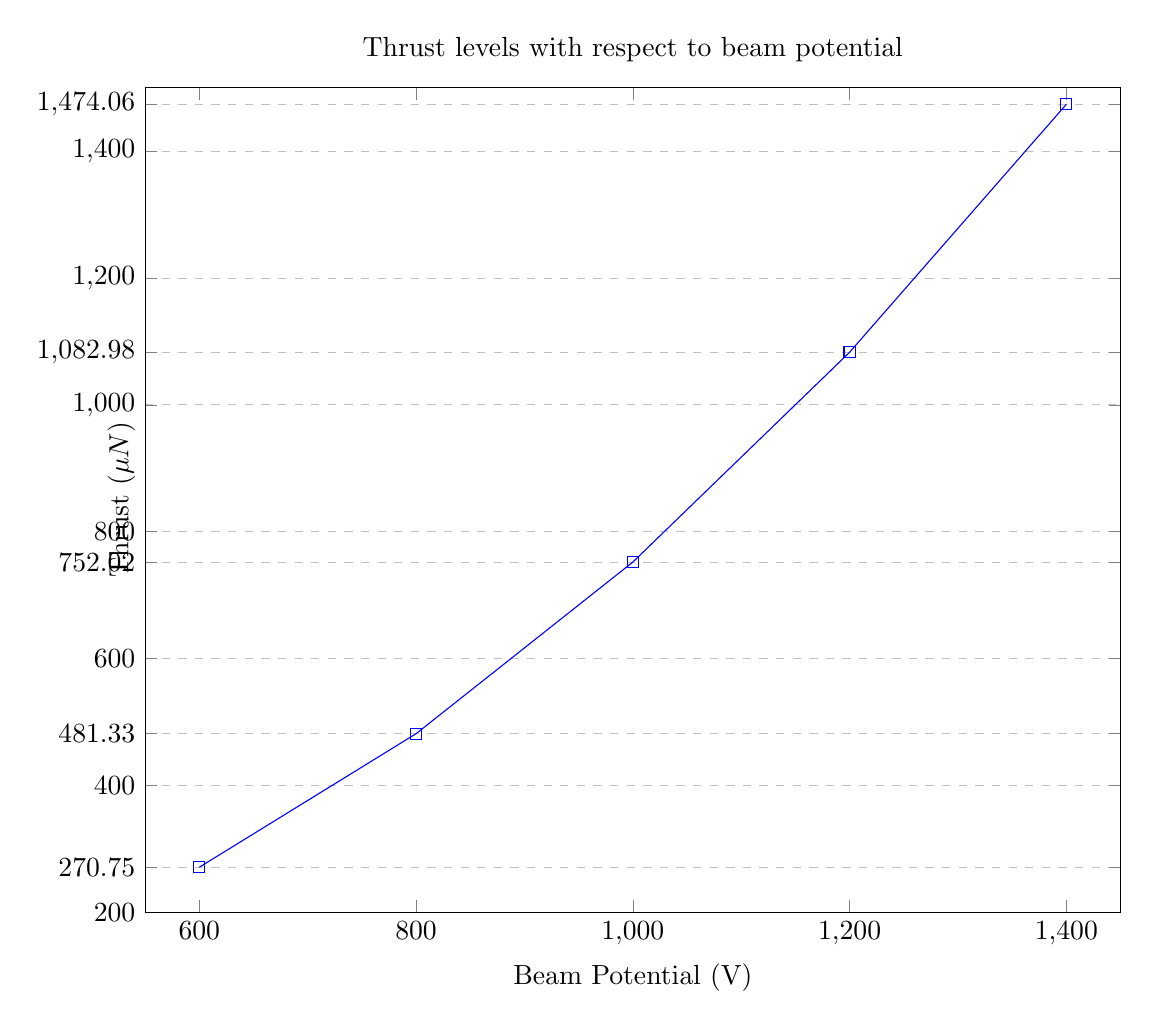
\begin{tikzpicture}
    \pgfplotsset{width=5.5in}
    \begin{axis}[
        title={Thrust levels with respect to beam potential},
        xlabel={Beam Potential (V)},
        y label style={at={(axis description cs:0,.5)}, anchor=south},
        ylabel={Thrust ($\mu N$)},
        xmin=550, xmax=1450,
        ymin=200, ymax=1500,
        xtick={600, 800, 1000, 1200, 1400},
        ytick={200, 270.75, 400, 481.33, 600, 752.02, 800, 1000, 1082.98, 1200, 1400, 1474.06},
        legend pos=north west,
        ymajorgrids=true,
        grid style=dashed,
    ]
        \addplot[
        color=blue,
        mark=square,
        ]
        coordinates {
        (600,270.75)(800,481.33)(1000,752.02)(1200,1082.98)(1400,1474.06)
        };
    \end{axis}
    \end{tikzpicture}
    \caption{Thrust Levels With Respect to Beam Potential}
    \label{chart:thrustlevels}
\end{figure}

As can be seen in figure \ref{chart:thrustlevels} provided thrust levels increase exponentially with increasing beam voltage. 

\newpage
\subsection{Specific Impulse Calculations}

Specific impulse value is given as 

\begin{equation}
    I_{sp} = \gamma \frac{\eta_m}{g} \sqrt{\frac{2qV_b}{m_i}}
\end{equation}

Inserting the values of $\gamma$, $g$ and $q$;

\begin{equation}
    I_{sp} = 1.417 \times 10^3 \eta_m \sqrt{\frac{V_B}{m_i}}
\end{equation}

where $\eta_m$ is the mass utilization efficiency; ratio of ionized propellant to unionized propellant. Similar to thrust calculations assumptions are; doubly charged ion ratio is  as 10\%, ion beam divergence of 10 degrees and 850V beam voltage with argon propellant. Calculated specific impulse values with respect to mass utilization efficiency and beam potential is shown in figure \ref{chart:isplevels}

\begin{figure}[ht]
    \centering   
    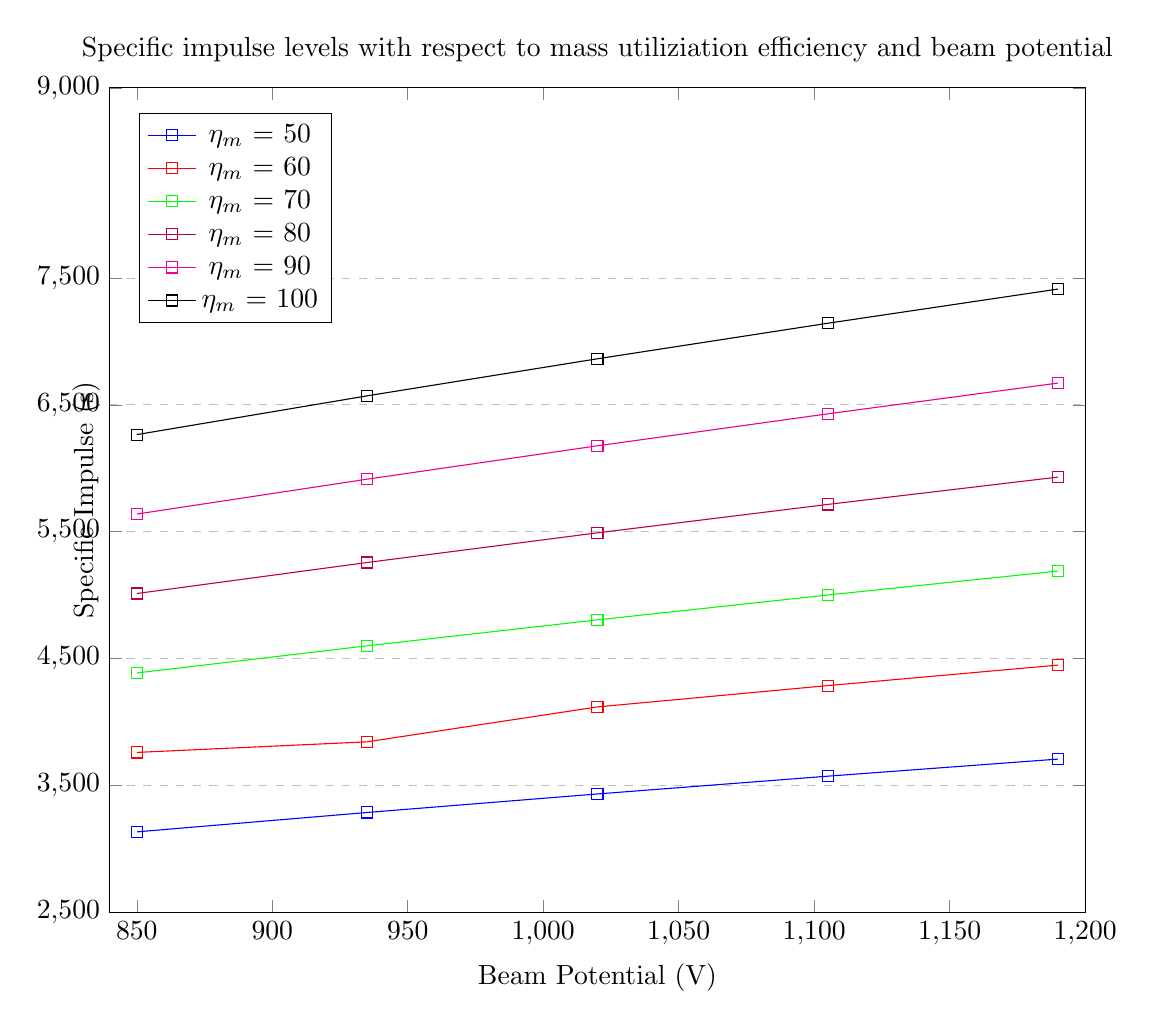
\begin{tikzpicture}
        \pgfplotsset{width=5.5in}
        \begin{axis}
            [
            title={Specific impulse levels with respect to mass utiliziation efficiency and beam potential},
            xlabel={Beam Potential (V)},
            y label style={at={(axis description cs:0,.5)}, anchor=south},
            ylabel={Specific Impulse (s)},
            xmin=840, xmax=1200,
            ymin=2500, ymax=9000,
            xtick={800, 850, 900, 950, 1000, 1050, 1100, 1150, 1200},
            ytick={2500, 3500, 4500, 5500, 6500, 7500, 9000},
            legend pos=north west,
            ymajorgrids=true,
            grid style=dashed,
        ]
            \addplot[
            color=blue,
            mark=square,
            ]
            coordinates {
            (850,3132.77)(935,3285.68)(1020,3431.78)(1105,3571.91)(1190,3706.74)
            };
            \addlegendentry{$\eta_m$ = 50}
            \addplot[
            color=red,
            mark=square,
            ]
            coordinates {
            (850,3759.32)(935,3842.81)(1020,4118.13)(1105,4286.29)(1190,4448.09)
            };
            \addlegendentry{$\eta_m$ = 60}
            \addplot[
            color=green,
            mark=square,
            ]
            coordinates {
            (850,4385.88)(935,4599.95)(1020,4804.49)(1105,5000.67)(1190,5189.44)
            };
            \addlegendentry{$\eta_m$ = 70}
            \addplot[
                color=purple,
                mark=square,
                ]
                coordinates {
                (850,5012.43)(935,5257.08)(1020,5490.84)(1105,5715.05)(1190,5930.79)
                };
                \addlegendentry{$\eta_m$ = 80}
                \addplot[
                    color=magenta,
                    mark=square,
                    ]
                    coordinates {
                    (850,5638.98)(935,5914.22)(1020,6177.2)(1105,6429.43)(1190,6672.14)
                    };
                    \addlegendentry{$\eta_m$ = 90}
                    \addplot[
                        color=black,
                        mark=square,
                        ]
                        coordinates {
                        (850,6265.54)(935,6571.35)(1020,6863.55)(1105,7143.81)(1190,7413.48)
                        };
                        \addlegendentry{$\eta_m$ = 100}
        \end{axis}
        \end{tikzpicture}
        \caption{$I_{sp}$ levels with respect to $\eta_m$ and $V_B$}
        \label{chart:isplevels}
    \end{figure}
    



% \subsection{1st Prototype}
% \subsection{2nd Prototype}

 
% \subsection{Page Margins}


% The gap at the bottom of the page is 2.5 cm. 

% Keeping more redundant space is incorrect. So, this gap should not be. Texts, tables, figures, etc. in the pages must be arranged considering this situation.

% \section{RF System Design}




% % ---------------------------------------------------------------- %
% % Numbered citation.						                       %
% % ---------------------------------------------------------------- %

